\documentclass[]{book}
\usepackage{lmodern}
\usepackage{amssymb,amsmath}
\usepackage{ifxetex,ifluatex}
\usepackage{fixltx2e} % provides \textsubscript
\ifnum 0\ifxetex 1\fi\ifluatex 1\fi=0 % if pdftex
  \usepackage[T1]{fontenc}
  \usepackage[utf8]{inputenc}
\else % if luatex or xelatex
  \ifxetex
    \usepackage{mathspec}
  \else
    \usepackage{fontspec}
  \fi
  \defaultfontfeatures{Ligatures=TeX,Scale=MatchLowercase}
\fi
% use upquote if available, for straight quotes in verbatim environments
\IfFileExists{upquote.sty}{\usepackage{upquote}}{}
% use microtype if available
\IfFileExists{microtype.sty}{%
\usepackage{microtype}
\UseMicrotypeSet[protrusion]{basicmath} % disable protrusion for tt fonts
}{}
\usepackage[margin=1in]{geometry}
\usepackage{hyperref}
\hypersetup{unicode=true,
            pdftitle={Gridded GDP projections compatible with the five SSPs},
            pdfauthor={Global Carbon Project (Tsukuba International Office), NIES and ISM, Japan},
            pdfborder={0 0 0},
            breaklinks=true}
\urlstyle{same}  % don't use monospace font for urls
\usepackage{natbib}
\bibliographystyle{apalike}
\usepackage{longtable,booktabs}
\usepackage{graphicx,grffile}
\makeatletter
\def\maxwidth{\ifdim\Gin@nat@width>\linewidth\linewidth\else\Gin@nat@width\fi}
\def\maxheight{\ifdim\Gin@nat@height>\textheight\textheight\else\Gin@nat@height\fi}
\makeatother
% Scale images if necessary, so that they will not overflow the page
% margins by default, and it is still possible to overwrite the defaults
% using explicit options in \includegraphics[width, height, ...]{}
\setkeys{Gin}{width=\maxwidth,height=\maxheight,keepaspectratio}
\IfFileExists{parskip.sty}{%
\usepackage{parskip}
}{% else
\setlength{\parindent}{0pt}
\setlength{\parskip}{6pt plus 2pt minus 1pt}
}
\setlength{\emergencystretch}{3em}  % prevent overfull lines
\providecommand{\tightlist}{%
  \setlength{\itemsep}{0pt}\setlength{\parskip}{0pt}}
\setcounter{secnumdepth}{5}
% Redefines (sub)paragraphs to behave more like sections
\ifx\paragraph\undefined\else
\let\oldparagraph\paragraph
\renewcommand{\paragraph}[1]{\oldparagraph{#1}\mbox{}}
\fi
\ifx\subparagraph\undefined\else
\let\oldsubparagraph\subparagraph
\renewcommand{\subparagraph}[1]{\oldsubparagraph{#1}\mbox{}}
\fi

%%% Use protect on footnotes to avoid problems with footnotes in titles
\let\rmarkdownfootnote\footnote%
\def\footnote{\protect\rmarkdownfootnote}

%%% Change title format to be more compact
\usepackage{titling}

% Create subtitle command for use in maketitle
\newcommand{\subtitle}[1]{
  \posttitle{
    \begin{center}\large#1\end{center}
    }
}

\setlength{\droptitle}{-2em}

  \title{Gridded GDP projections compatible with the five SSPs}
    \pretitle{\vspace{\droptitle}\centering\huge}
  \posttitle{\par}
    \author{Global Carbon Project (Tsukuba International Office), NIES and ISM, Japan}
    \preauthor{\centering\large\emph}
  \postauthor{\par}
      \predate{\centering\large\emph}
  \postdate{\par}
    \date{February, 2020}

\usepackage{booktabs}
\usepackage{amsthm}
\makeatletter
\def\thm@space@setup{%
  \thm@preskip=8pt plus 2pt minus 4pt
  \thm@postskip=\thm@preskip
}
\makeatother

\begin{document}
\maketitle

{
\setcounter{tocdepth}{1}
\tableofcontents
}
\hypertarget{downscaling-gdp}{%
\chapter*{Downscaling GDP}\label{downscaling-gdp}}
\addcontentsline{toc}{chapter}{Downscaling GDP}

Historical and future spatially explicit population and GDP data are critically important for analysing climate risks in the future. Population projection exists such as HYDE database, but GDP projection does not exist especially SSP compatible scenarios. So, we have estimated GDP with 1/12-degree grid-scale during 1850---2100 by 10 year intervals. National GDP data was downscaled to grids using the past data until 2010 and future data until 2100 of SSPs. In the downscaling algorithm, we first assumed spatial and economic interactions among cities and projected future different urban growth patterns according to SSPs. Then, the projected urban growth patterns and other auxiliary geographic data (land cover, road network, etc.) were used to estimate the gridded GDP distributions. Finally, the estimated GDPs were visualized in 3D for the intuitive understanding for multiple stakeholders. Our results suggested that spatial pattern of urban and peri-urban GDP could change considerably depending on SSPs. For example, GDP of SSP1 shows rapid urban growth nearby major cities while SSP3 shows lower level of urban growth nearby the cities, and SSP5 shows extreme urban dispersion.

Methods which we used are detaily described in our forthcoming paper:
\textbf{Murakami, Yoshida, and Yamagata (202X)}. Please see the reference section below.

\begin{figure}
\centering
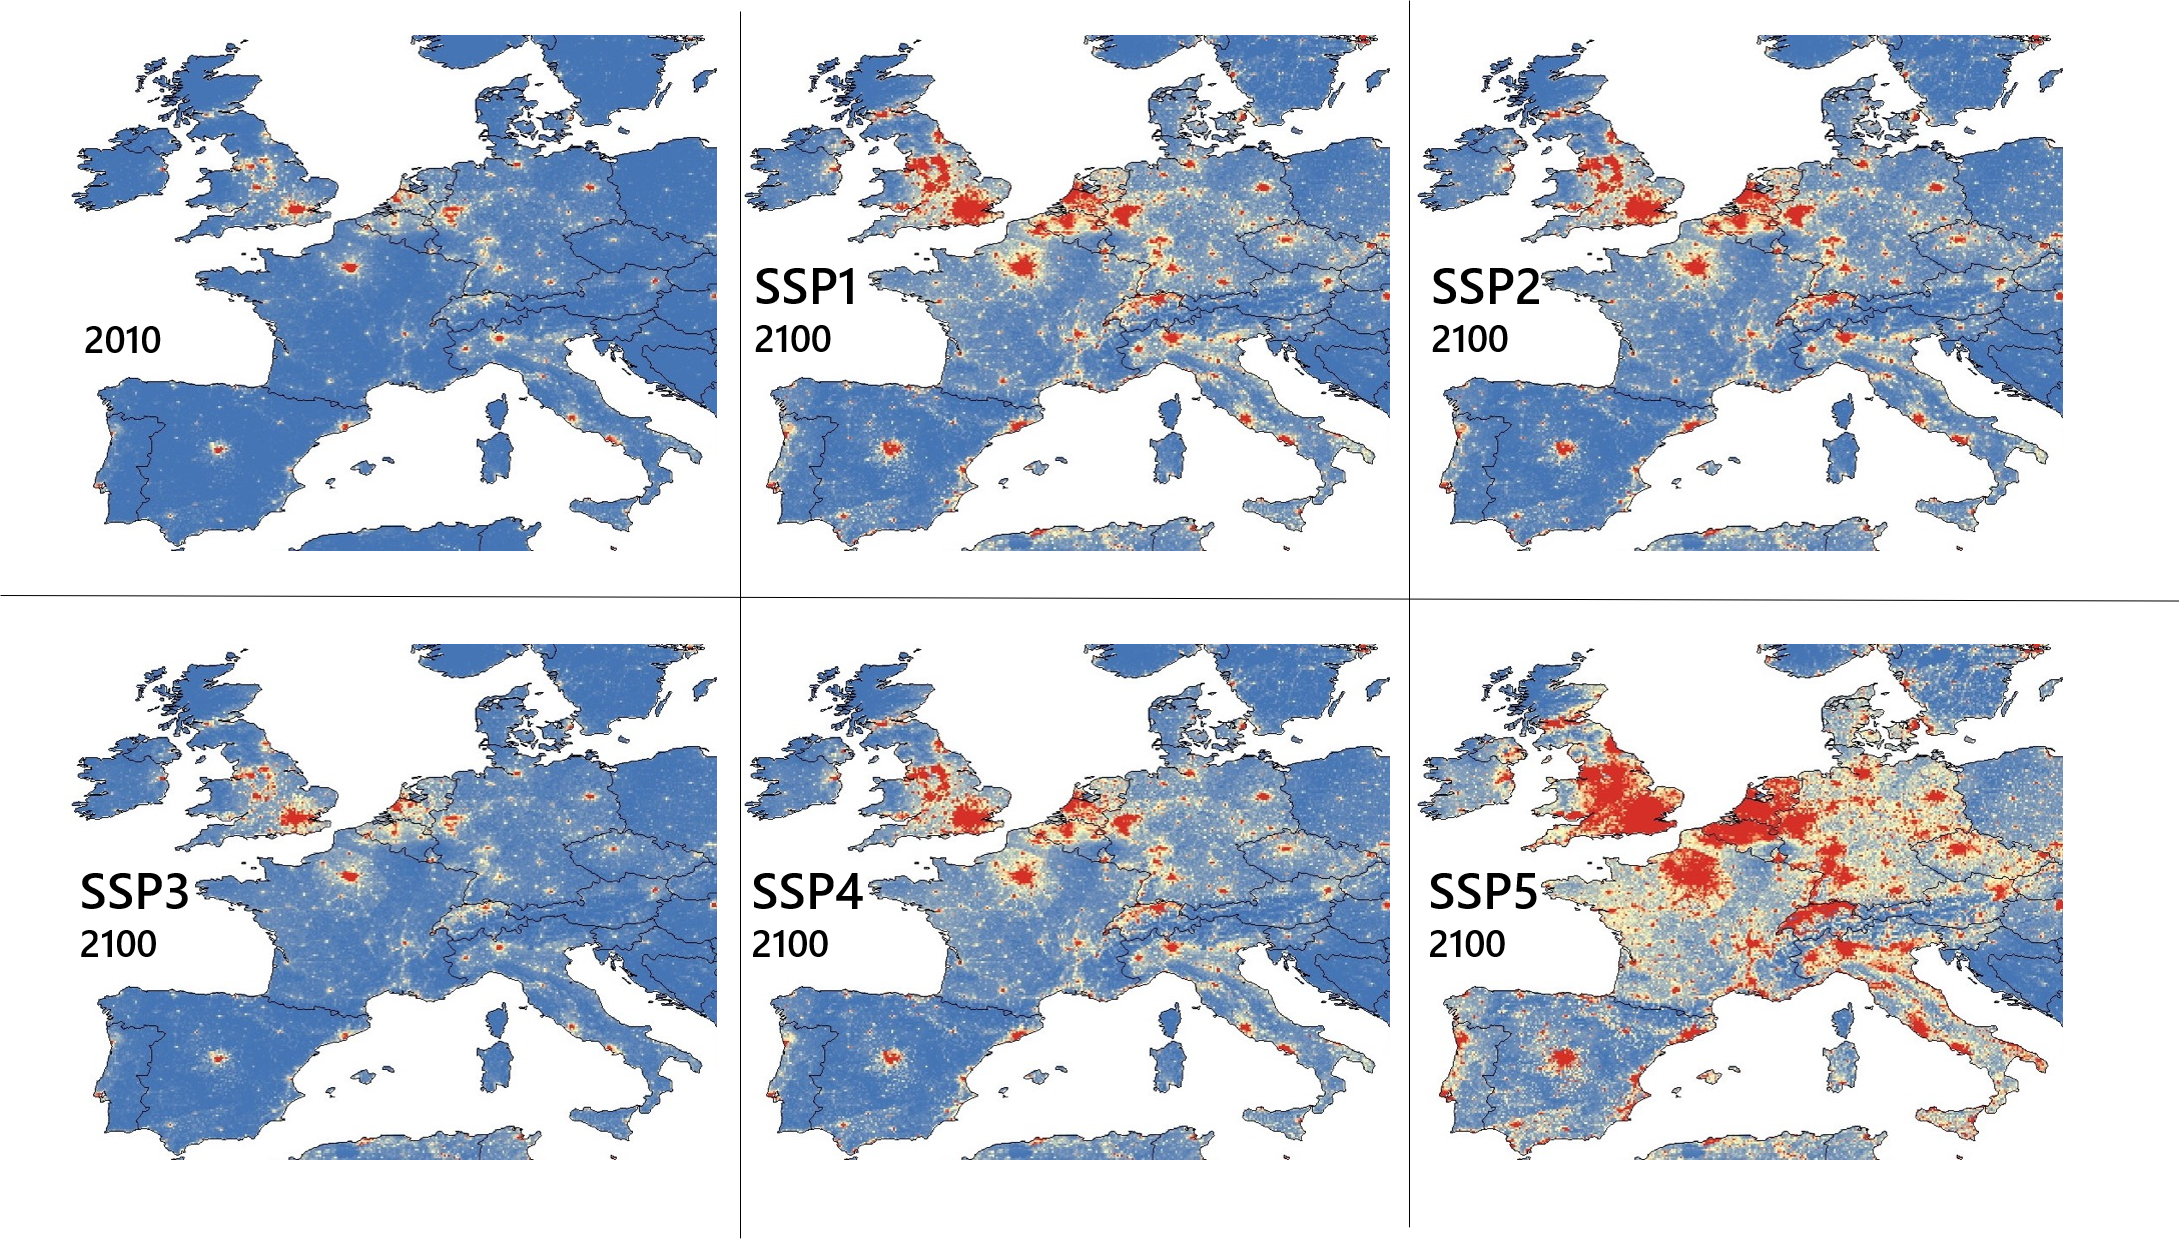
\includegraphics{Europe.png}
\caption{Figure: Europe in 2D}
\end{figure}

\begin{figure}
\centering
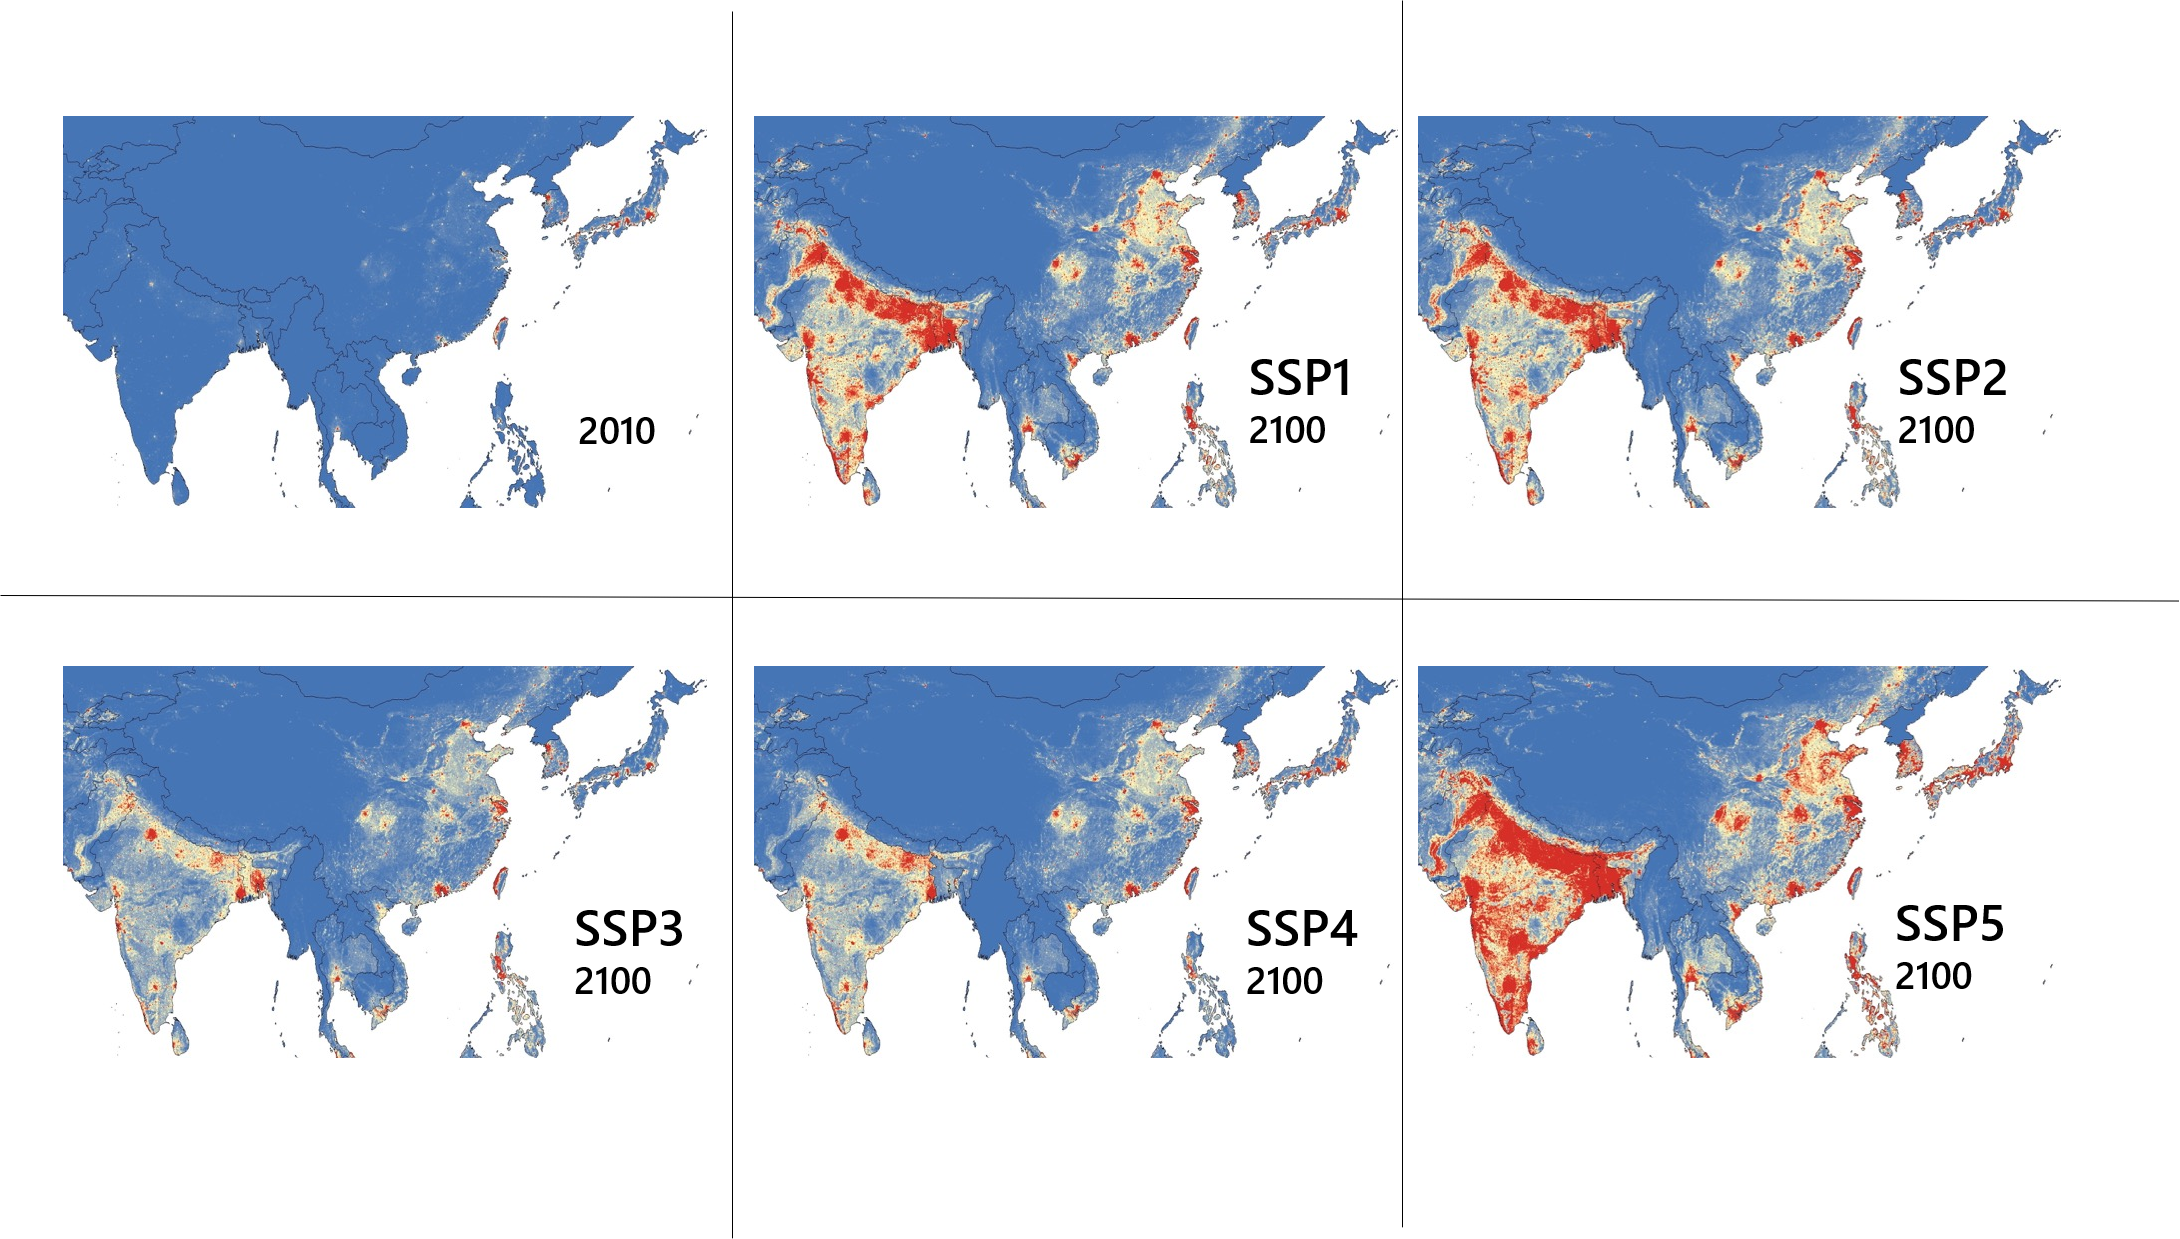
\includegraphics{Asia.png}
\caption{Figure: Asia in 2D}
\end{figure}

\begin{verbatim}
## PhantomJS not found. You can install it with webshot::install_phantomjs(). If it is installed, please make sure the phantomjs executable can be found via the PATH variable.
\end{verbatim}

\hypertarget{g1RR7JrsS2}{}

Figure: Interactive 3D globe maping on downscaled GDP in 2000. You can pan and zoom the globe by mouse-over.

\begin{center}\rule{0.5\linewidth}{\linethickness}\end{center}

\hypertarget{data-download}{%
\section*{Data download}\label{data-download}}
\addcontentsline{toc}{section}{Data download}

The GDPs for SSP 1--5 between 2000 and 2100 by 10 years are estimated by 2160 x 4320 grids, each of which are 1/12-degree grids, covering the globe. The GDP estimates in each year in each SSP are recorded as a GeoTIff image with resolution of 2160 x 4320. GeoTiff is a Tiff image with spatial coordinates for each grid cell; the coordinates are given by longitude and latitude measured by World Geodetic System 1984 (WGS84).

\textbf{\emph{please click here: tiff and csv files}} (please wait a moment.)

And also, you can download 3D globemap html files on the five SSPs (2000-2100) from the link below.

\textbf{\emph{please click here: 3D globemaps}} (please wait a moment.)

\begin{center}\rule{0.5\linewidth}{\linethickness}\end{center}

\hypertarget{code-for-visualization}{%
\section*{Code for visualization}\label{code-for-visualization}}
\addcontentsline{toc}{section}{Code for visualization}

We used \href{https://www.r-project.org/}{\textbf{R}} for the 3D globe visualization.

\begin{verbatim}
library(colorRamps)
library(data.table)
library(dplyr)
library(htmlwidgets)
library(threejs)
library(tidyr)

setwd(****) # please set a directory including the file
dat <- fread(****) # please wait a moment!
# dat[1:3,]
#    longitude latitude gdp
# 1: -36.54172  83.5416   *
# 2: -36.45839  83.5416   *
# 3: -36.37506  83.5416   *

dat <- dat %>%
       mutate(gdp=if_else(gdp>0,gdp,0)) %>%
       filter(gdp>0) %>%
       mutate(gdp.cut=as.numeric(cut(gdp,
        breaks=c(0,10^4,10^5,10^6,2.5*10^6,5.0*10^6,
                 10^7,2.5*10^7,5.0*10^7,10^8,10^9,max(gdp)), 
        include.lowest=TRUE))) %>%
       mutate(pid=as.numeric(rownames(.))%%10) %>% # to avoid heavy calculation.
       filter(pid==0)
3Dglobe <- globejs(lat=dat$latitude, long=dat$longitude,
        val=dat$gdp/70000000, # to adjust bar height 
        color=matlab.like(11)[dat$gdp.cut],
        pointsize=1.6,
        atmosphere=F)
3Dglobe        
\end{verbatim}

\begin{center}\rule{0.5\linewidth}{\linethickness}\end{center}

\hypertarget{references}{%
\section*{References}\label{references}}
\addcontentsline{toc}{section}{References}

\begin{itemize}
\tightlist
\item
  Daisuke Murakami, Takahiro Yoshida, Yoshiki Yamagata (202X) \textbf{Gridded GDP projections compatible with the five SSPs (Shared Socioeconomic Pathways)}. Submitted to \emph{a journal}.
\end{itemize}

\bibliography{book.bib,packages.bib}


\end{document}
